\documentclass{ifacconf}

\usepackage{natbib}            % you should have natbib.sty
\usepackage[utf8]{inputenc}    % Eingabe von Umlauten im Editor, dieser sollte dann auch auf utf8 Encoding eingestellt sein
\usepackage{graphicx}          % Include this line if your 
                               % document contains figures,
%\usepackage[dvips]{epsfig}    % or this line, depending on which
                               % you prefer.
\usepackage{multirow}
                               
\usepackage{units}
\usepackage{amssymb}
\usepackage{gensymb}
\usepackage{float}
% for German
% \usepackage{ngerman}           % neue Deutsche Rechtschreibung, Silbentrennung
% \usepackage[T1]{fontenc}       % Trennung mit Umlauten

% to include tikz pictures of figure created with matlab2tikz, see also file ``plotFigureTest.m''
\usepackage{tikz}
\usepackage{pgfplots}
\pgfplotsset{compat=newest}  % use newest version of pgfplots
\usepackage{amsmath}  % useful for math

% to include the legend into the caption. The commands are
%\mlLineLegend{red}
%\mlLineLegendDashed{red}
%\mlLineLegendDotted{red}
%\mlLineLegendDashDotted{red}
%\mlPointLegend{red}
\newlength{\mlLegendThickness}
\setlength{\mlLegendThickness}{0.4mm}
\newlength{\mlLegendHeight}
\setlength{\mlLegendHeight}{0.6ex}
\newcommand{\mlLineLegend}[1]{\mbox{\color{#1}
\protect\rule[\mlLegendHeight]{3mm}{\mlLegendThickness}\hspace*{-1mm}
}}
\newcommand{\mlLineLegendDashed}[1]{\mbox{\color{#1}
\protect\rule[\mlLegendHeight]{1.5mm}{\mlLegendThickness}\hspace*{0mm}
\protect\rule[\mlLegendHeight]{1.5mm}{\mlLegendThickness}\hspace*{-1mm}
}}
\newcommand{\mlLineLegendDotted}[1]{\mbox{\color{#1}
\protect\rule[\mlLegendHeight]{0.4mm}{\mlLegendThickness}\hspace*{0mm}
\protect\rule[\mlLegendHeight]{0.4mm}{\mlLegendThickness}\hspace*{0mm}
\protect\rule[\mlLegendHeight]{0.4mm}{\mlLegendThickness}\hspace*{0mm}
\protect\rule[\mlLegendHeight]{0.4mm}{\mlLegendThickness}\hspace*{-1mm}
}}
\newcommand{\mlLineLegendDashDotted}[1]{\mbox{\color{#1}
\protect\rule[\mlLegendHeight]{1.5mm}{\mlLegendThickness}\hspace*{0mm}
\protect\rule[\mlLegendHeight]{0.4mm}{\mlLegendThickness}\hspace*{0mm}
\protect\rule[\mlLegendHeight]{1.5mm}{\mlLegendThickness}\hspace*{0mm}
\protect\rule[\mlLegendHeight]{0.4mm}{\mlLegendThickness}\hspace*{-1mm}
}}
\newcommand{\mlPointLegend}[1]{\mbox{\color{#1}
\protect\rule[\mlLegendHeight]{0.4mm}{\mlLegendThickness}\hspace*{-0.75mm}
}}

\begin{document}

\begin{frontmatter}
	
\title{Gruppe B-Mo2: \\ Abschlussprotokoll des KRT Praktikums}
% include all authors, underline corresponding author
\author{Yuchan Bian,} 
\author{Jiaqi Qin,}
\author{E. Boateng} 


\begin{abstract}                          % Abstract of not more than 250 words.
Das vorliegende Protokoll beschreibt das Vorgehen des Praktikums Konzept der Regelungstechnik. Im Praktikum wird an einem 3-DOF Helikopter eine Regelungsaufgabe systematisch gelöst. Der Helikopter muss eine Trajektorie mit Beschränkungen wie Mindesthöhe abfliegen und eine Last von einem
Landepunkt zu einem anderen transportieren. Die Modellierung des Systems erfolgte mithilfe des Drallsatzes. Das resultierende nichtlineare Modell wird um einen Arbeitspunkt linearisiert. Mittels des lineariserten Modells wird ein LQI-Regler entworfen. Die Erfüllung der Hauptaufgabe wird dann mit einer geplanten Solltrajektorie durchgeführt. Abschließend wurden die Reglerparameter optimiert, um ein gutes Ergebnis zu erzielen.
\end{abstract}

\end{frontmatter}

\section{Einleitung}
Dieses Protokoll ist die Zusammenfassung der durchgefuehrten Schritte zur erfolgreichen Absolvierung des Praktikums im WS 20/21. Im ersten Kapitel wird die Aufgabestellung und der Versuchsaufbau vorgestellt. Anschließend wird die Modellierung und die Auslegung des Reglers beschrieben. Zuletzt wird das Ergebnis gezeigt.

\subsection{Aufgabenstellung}
Ziel des Praktikums ist, wie in Abbildung 1 dargestellt, einen automatisierten Lastentransport zu realisieren. Der Helikopter soll die Aufgabe automatisch lösen können und dabei Mindesthöhen einhalten.

\subsection{Versuchsaufbau}
Der Versuchsaufbau ist in Abbildung 2 dargestellt. Darin wird das Koordinatensystem und die dazugehörigen Winkel definiert. Die Drehung um die $x$-Achse (Schwenkwinkel), $y$-Achse (Steigwinkel) und $z$-Achse (Nickwinkel) sind jeweils mit \alpha, \beta und \gamma bezeichnet. Der Helikopter verfügt über die zwei einzeln ansteuerbare Motoren (Frontmotor und Heckmotor). Die zugehörigen Spannungen werden entsprechend mit $U_F$ und $U_B$ bezeichnet.

\begin{figure}
	\begin{center} 
		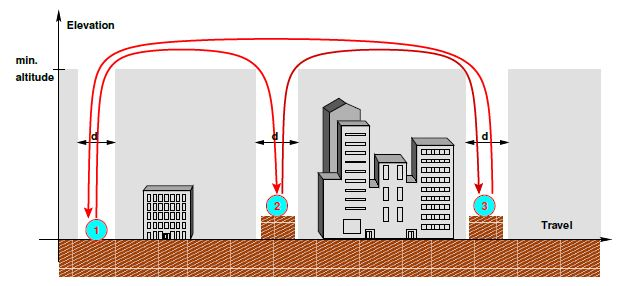
\includegraphics[scale=0.7]{hauptaufgabe} 
		\caption{Flugbahn der Hauptaufgabe}
		\label{fig:hauptaufgabe}
	\end{center}
	
	\begin{center} 
		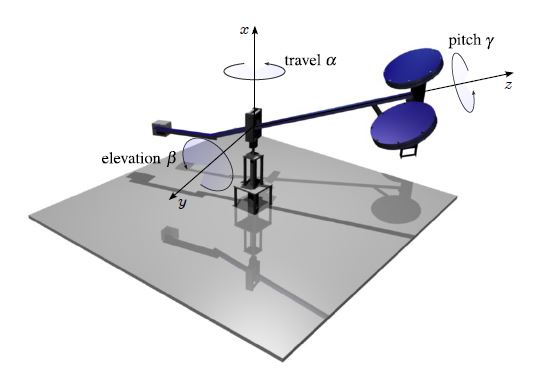
\includegraphics[scale=0.7]{koordinatensystem} 
		\caption{Darstellung des Versuchsaufbaus}
		\label{fig:koordinatensystem}
	\end{center}
\end{figure}


\section{Modellierung}
Der Reglerentwurf erfolgte anhand eines modellierten System des Helikopters. Um die Komplexitätsgrad bei der Modellierung zu reduzieren wurden folgenden Annahmen verwendet.
\begin{enumerate}
\item Alle Lager wurden als ideal angenommen.
\item Die Geometrien der einzelnen Komponenten wurden als starr und ideal angesehen
\item Alle Massen drehen sich symmetrisch um die verschiedenen Drehachsen
\item Die Rotation aller Massen erfolgt um den Schwerpunkt
\end{enumerate}

%Figure 1 shows the simplified model with the corresponding
%parameters.
%
%Applying the law of angular momentum to the axes a, b and c, the following equations are derived.
Unter Anwendung des Drehimpulssatzs auf die Achsen a, b und c wurde folgenden Gleichungen abgeleitet

%\break 
\begin{align}	
&\Theta_a\ddot{\alpha} = -\cos(\beta)L_2\sin(\gamma)(F_f+F_b)\\
&\Theta_b\ddot{\beta} = \cos(\gamma)L_2(F_f+F_b)-\cos(\beta)(mL_1-ML_2)g\\
&\Theta_c\ddot{\gamma} = \frac{L_3}{2}(F_f-F_b)
\end{align}

%$\Theta_a$, $\Theta_b$ and $\Theta_c$ sind jeweils die Trägheitsmomenten in Bezug auf die Achsen a, b und c. 

%\break
Mit 
\begin{align}
\Theta_a &= mL_1^2 + ML_2^2\\
\Theta_b &= mL_1^2 + ML_2^2\\
\Theta_c &= \frac{mL_3^2}{24}
\end{align}

\begin{figure} % use \begin{figure*} for two-column figure
\begin{center} 
% the variable for the width of the figure which you created with matlab2tikz has to be defined and set
\newlength{\figurewidth} % ... defined
\setlength{\figurewidth}{0.5\columnwidth} % ...set 
% for details see file ``plotFigureTest.m''
%% This file was created by matlab2tikz.
%
%The latest updates can be retrieved from
%  http://www.mathworks.com/matlabcentral/fileexchange/22022-matlab2tikz-matlab2tikz
%where you can also make suggestions and rate matlab2tikz.
%
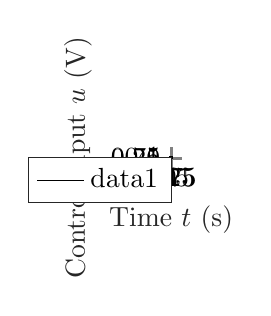
\begin{tikzpicture}

\begin{axis}[%
width=0.951\figurewidth,
height=0.75\figurewidth,
at={(0\figurewidth,0\figurewidth)},
scale only axis,
xmin=0,
xmax=1,
xtick={   0, 0.25,  0.5, 0.75,    1},
xlabel style={font=\color{white!15!black}},
xlabel={Time $t$ (s)},
ymin=0,
ymax=1,
ytick={   0, 0.25,  0.5, 0.75,    1},
ylabel style={font=\color{white!15!black}},
ylabel={Control input $u$ (V)},
axis background/.style={fill=white},
xmajorgrids,
ymajorgrids,
legend style={legend cell align=left, align=left, draw=white!15!black}
]
\addplot [color=black]
  table[row sep=crcr]{%
0	0\\
0.01	0.00999983333416666\\
0.02	0.0199986666933331\\
0.03	0.0299955002024957\\
0.04	0.0399893341866342\\
0.05	0.0499791692706783\\
0.06	0.0599640064794446\\
0.07	0.0699428473375328\\
0.08	0.0799146939691727\\
0.09	0.089878549198011\\
0.1	0.0998334166468282\\
0.11	0.109778300837175\\
0.12	0.119712207288919\\
0.13	0.129634142619695\\
0.14	0.139543114644236\\
0.15	0.149438132473599\\
0.16	0.159318206614246\\
0.17	0.169182349066996\\
0.18	0.179029573425824\\
0.19	0.188858894976501\\
0.2	0.198669330795061\\
0.21	0.2084598998461\\
0.22	0.218229623080869\\
0.23	0.227977523535188\\
0.24	0.237702626427135\\
0.25	0.247403959254523\\
0.26	0.257080551892155\\
0.27	0.266731436688831\\
0.28	0.276355648564114\\
0.29	0.285952225104836\\
0.3	0.29552020666134\\
0.31	0.305058636443443\\
0.32	0.314566560616118\\
0.33	0.324043028394868\\
0.34	0.333487092140814\\
0.35	0.342897807455451\\
0.36	0.35227423327509\\
0.37	0.361615431964962\\
0.38	0.370920469412983\\
0.39	0.380188415123161\\
0.4	0.389418342308651\\
0.41	0.398609327984423\\
0.42	0.40776045305957\\
0.43	0.416870802429211\\
0.44	0.425939465066\\
0.45	0.43496553411123\\
0.46	0.44394810696552\\
0.47	0.452886285379068\\
0.48	0.461779175541483\\
0.49	0.470625888171158\\
0.5	0.479425538604203\\
0.51	0.488177246882908\\
0.52	0.496880137843737\\
0.53	0.505533341204847\\
0.54	0.514135991653113\\
0.55	0.522687228930659\\
0.56	0.531186197920883\\
0.57	0.539632048733969\\
0.58	0.548023936791874\\
0.59	0.556361022912784\\
0.6	0.564642473395035\\
0.61	0.572867460100481\\
0.62	0.581035160537305\\
0.63	0.58914475794227\\
0.64	0.597195441362392\\
0.65	0.605186405736039\\
0.66	0.613116851973434\\
0.67	0.62098598703656\\
0.68	0.628793024018468\\
0.69	0.636537182221968\\
0.7	0.644217687237691\\
0.71	0.651833771021537\\
0.72	0.659384671971473\\
0.73	0.666869635003698\\
0.74	0.674287911628145\\
0.75	0.681638760023334\\
0.76	0.688921445110551\\
0.77	0.696135238627357\\
0.78	0.70327941920041\\
0.79	0.710353272417608\\
0.8	0.717356090899523\\
0.81	0.724287174370143\\
0.82	0.731145829726896\\
0.83	0.737931371109963\\
0.84	0.744643119970859\\
0.85	0.751280405140293\\
0.86	0.757842562895277\\
0.87	0.764328937025505\\
0.88	0.770738878898969\\
0.89	0.777071747526824\\
0.9	0.783326909627483\\
0.91	0.78950373968995\\
0.92	0.795601620036366\\
0.93	0.801619940883777\\
0.94	0.807558100405114\\
0.95	0.813415504789374\\
0.96	0.819191568300998\\
0.97	0.82488571333845\\
0.98	0.83049737049197\\
0.99	0.836025978600521\\
1	0.841470984807897\\
};
\addlegendentry{data1}

\end{axis}
\end{tikzpicture}% % inclusion of tikz-code
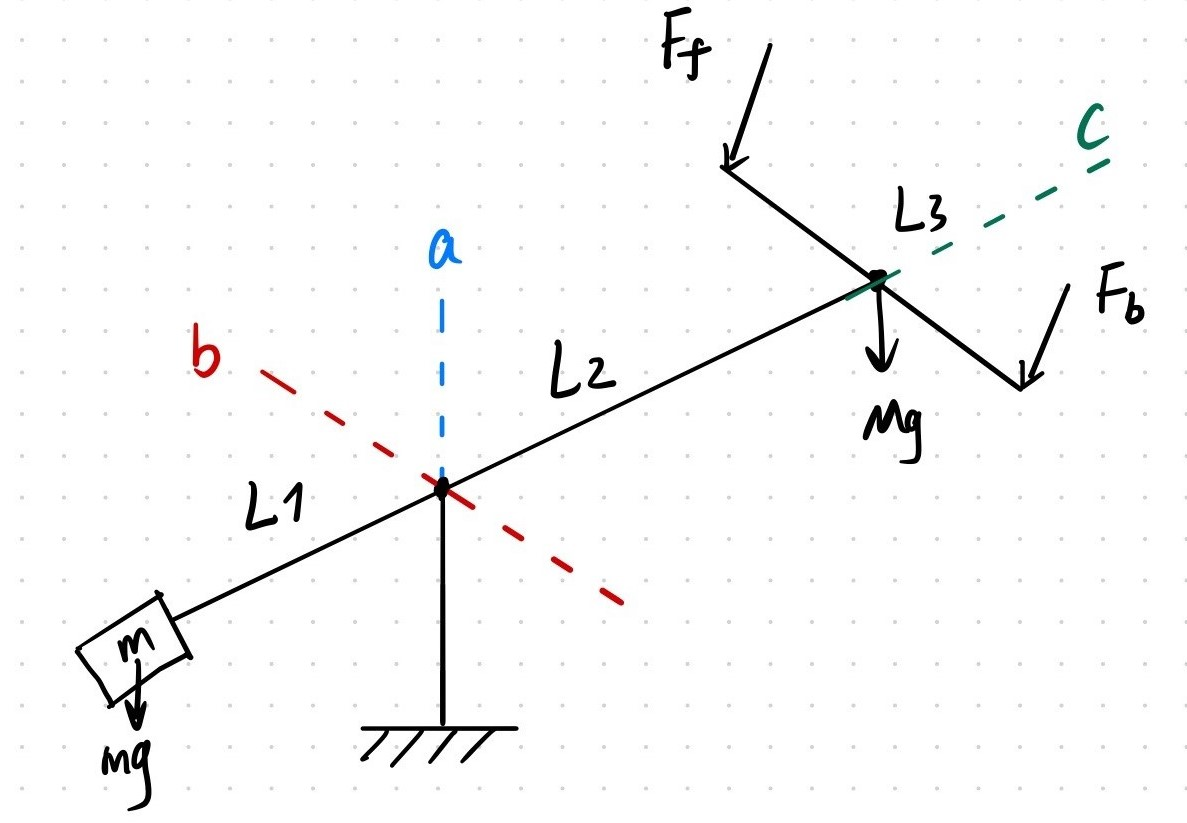
\includegraphics[width=\columnwidth]{model} % inclusion of pdf
\caption{vereinfachtes Modell des Hubschraubersr}
\label{model}
\end{center}
\end{figure}


Der Zustandsvektor $x =\begin{bmatrix}
	\alpha&\beta&\gamma&\dot{\alpha}&\dot{\beta}&\dot{\gamma}
\end{bmatrix}^T$ und der Eingangsvektor $u = \begin{bmatrix}
F_f&F_b
\end{bmatrix}^T$. Es folgt daraus dass, 
\begin{equation}
\dot{x}=\begin{bmatrix}
	\dot{\alpha}\\[0.5 em]
	\dot{\beta}\\[0.5 em]
	\dot{\gamma}\\[0.5 em]
	\frac{-\cos(\beta)L_2\sin(\gamma)(F_f+F_b)}{mL_1^2 + ML_2^2}\\[1.2 em]
	\frac{\cos(\gamma)L_2(F_f+F_b)-\cos(\beta)(mL_1-ML_2)g}{mL_1^2 + ML_2^2}\\[1.2 em]
	\frac{12(F_f-F_b)}{mL_3}
\end{bmatrix}
\end{equation}

Die bereitgestellte Helikopterdaten stellte die Beziehung zwischen der Spannung und der entsprechenden Änderung des Deltas der Massen dar. Mithilfe der Kurvenanpassungsbefehl \textit{polyfit} in Matlab konnte die Parameter der Kurve ermittelt.
Die berechnete Koeffizienten lautet:
\\
\begin{align}
	F_f (U) &= 6.156*10^{-2}\\ %U^2 \\ %-0.1342U 	-0.13917\\
	F_b (U) &= 4.704*10^{-2}  %U^2 	%+0.00510U 	-0.278
\end{align}

Unter Verwendung der Gleichungen des vereinfachten physikalischen Modells des Hubschraubers, die in bereits diskutiert wurde, wird das Zustandsraummodell der Regelstrecke abgeleitet.

$A_{lin}=
\left(\begin{array}{cccccc} 
\multicolumn{3}{c}{\multirow{3}{*}{\emph{O_{3,3}}}}& \multicolumn{3}{c}{\multirow{3}{*}{\emph{I_3}}}&\\
 &  &  &  &  & \\
 &  &  &  &  & \\
 &  &  &  &  & \\
%0 & 0 & 0 & 1.0 & 0 & 0\\
%0 & 0 & 0 & 0 & 1.0 & 0\\
%0 & 0 & 0 & 0 & 0 & 1.0\\
0 & 0 & \frac{0.887L_2 (F_f -F_b)}{\sigma_1 } & \multicolumn{3}{c}{\multirow{3}{*}{\emph{O_{3,3}}}} & & \\
0 & \frac{0.462ML_2g - mL_1g}{\sigma_1 } &0 & & & \\[1.5 em]
0 & 0 & 0 & & &
\end{array}\right)$\\[1.5 em]
{\text{mit  } $\sigma_1 = mL_1^2 + ML_2^2 $


$B_{lin} = \left(\begin{array}{cc}
\multicolumn{2}{c}{\multirow{4}{*}{\emph{O_{4,2}}}}\\[1.5 em]
 & \\
 & \\
\frac{L_2 }{mL_1^2 + ML_2^2 } & \frac{L_2 } {mL_1^2 +ML_2^2}\\[1.5 em]
\frac{12.0}{mL_3} & -\frac{12.0}{mL_3} \\
\end{array}\right)$

\subsection{Systemeigenschaften}
Beobachtbarkeit und Steuerbarkeit: Die Steuerbarkeit- und Beobachtbarkeitsmatrizen weisen einen vollen Rang auf. Dies deutet darauf dass das System beobachtbar und steuerbar ist. 
%++++++++

\section{Reglerentwurf}
\subsection{Reglerauswahl}
Durch die Aufgabenstellung der Trajektorien leiten sich die Zielvorgaben des Reglerentwurfs ab. Der Helikopter soll nicht nur stabilisiert werden sondern einer Trajektorienvorgabe möglichst robust und ohne Sollwertabweichung folgen. Zur Erfüllung der Aufgabenstellung werden an den Regler folgende Anforderung gestellt:
\begin{itemize}
	\item Der geschlossene Kreis soll stabil sein.
	\item  Die bleibende Regelabweichung von $\alpha$ und $\beta$  soll so gering sein, dass der Helikopter entlang einer vorgegebenen Trajektorie fliegen kann.
	\item Der Helikopter kann die vorgegebene Position schnell erreichen.
\end{itemize}
Ein LQR-Regler vereint diese Eigenschaften. Erweitert um einen I-Anteil, der eine Sollwertabweichung der Trajektorie minimiert, ist hier ein Ansatz zu einem LQI-Regelrentwurf beschrieben. Deshalb haben wir uns für einen LQI-Regler ausgewählt.

\subsection{Linearisierung}
Der Zustandsvektor x, die Schubkraft der Rotoren als Eingangsvektor u und der Ausgang y lauten wie folgend:
\begin{equation}
	x=\left[\begin{array}{c}
		\alpha,\beta,\gamma,\dot{\alpha},\dot{\beta},\dot{\gamma}\
	\end{array}\right]^T
\end{equation}
\begin{equation}
	u=\left[\begin{array}{c}
		F_{f}\\F_{b}
	\end{array}\right]
\end{equation}
\begin{equation}
	y=\left[\begin{array}{c}
		\alpha\\\beta\\\gamma
	\end{array}\right]
\end{equation}
Um das System leichter zu analysieren und die Basis fuer eine spaetere Regelerauslegung zu generieren, wird das System um eine Ruhelage linearisiert. Als Linearisierungspunkt wird
\begin{equation}
	\bar{x} =\left[\begin{array}{c}
		0,-3^{\circ},0,0,0,0
	\end{array}\right] ^{T}
\end{equation}
gewaehlt.
Auf Basis des Arbeitspunktes wird die Schubkraft als Eingang fuer die Ruhelage bestimmt. 
\begin{equation}
	\bar{u}=\left[\begin{array}{c}
		0.5873\\0.5873
	\end{array}\right]
\end{equation}

Für die Systemmatrix A ergibt sich durch Ableiten nach dem Zustandsvektor x und einsetzen des Linearisierungspunktes:
\begin{equation}
	A=\left[\begin{array}{llllll}
		0 & 0 & 0 & 1 & 0 & 0 \\
		0 & 0 & 0 & 0 & 1 & 0 \\
		0 & 0 & 0 & 0 & 0 & 1 \\
		0 & 0 & -0.6921& 0 & 0 & 0 \\
		0 & -0.0359& 0 & 0 & 0 & 0 \\
		0 & 0 & 0 & 0 & 0 & 0
	\end{array}\right]
\end{equation}
Die Eingangsmatrix B ergibt sich durch Jacobi-Matrix abgeleitet nach den Eingangsgrößen und einsetzen des Linearisierungspunktes zu:
\begin{equation}
	B=\left[\begin{array}{cc}
	\multicolumn{2}{c}{\multirow{4}{*}{\emph{O_{4,2}}}}\\
 			& \\
			& \\
		0.5832 & 0.5832\\
		5.5383& -5.5383\\
	\end{array}\right]
\end{equation}
Die Ausgangsmatrix C ergibt sich zu
\begin{equation}
	\begin{array}{l}
		C=\left[\begin{array}{llllll}
		\multicolumn{3}{c}{\multirow{3}{*}{\emph{I_3}}}& \multicolumn{3}{c}{\multirow{3}{*}{\emph{O_{3,3}}}}
			&  &  &  &  &  \\
			&  &  &  &  &  
%			1 & 0 & 0 & 0 & 0 & 0 \\
%			0 & 1 & 0 & 0 & 0 & 0 \\
%			0 & 0 & 1 & 0 & 0 & 0
		\end{array}\right] 
	\end{array}
\end{equation}

Die Durchgriffsmatrix D ergibt sich zu Null und ist mit folgender Dimension durch 

\begin{equation}
		D= O_{3,2}	
\end{equation}
%\begin{equation}
%	\begin{array}{l}
%		D= \left[\begin{array}{ll}
%%			0 & 0 \\
%%			0 & 0 \\
%%			0 & 0
%		\end{array}\right]
%	\end{array}
%\end{equation}
gegeben.\\

Bei weiteren Untersuchungen eines Beobachters und der Regelerauslegung ist darauf zu achten, dass das linearisierte Modell nun mit den Abweichungen $\Delta{x}$, $\Delta{u}$, $\Delta{y}$ der Größen arbeitet. 
 \begin{equation}{}
 	\Delta{x}=x-\bar{x},
 	\Delta{u}=u-\bar{u},
 	\Delta{y}=y-\bar{y}
 \end{equation}
Das linearisierte System ist vollständig gegeben durch:
\begin{equation}{}
	 \Delta{\dot{x}}=A \Delta{x}+B \Delta{u}  \qquad \Delta{y}=C\Delta{x}+ D \Delta{u} 
\end{equation}
mit der Anfangsbedingung 
 \begin{equation}{}
	\Delta{x}(0)=x(0)-\bar{x}
\end{equation}


%\subsection{Steuerbarkeit und Beobachtbarkeit}
%Die Steuerbarkeit und Beobachtbarkeit von Systemen sind in Matlab gerechnet und sie haben beiden Vollrank. Das lineare System ist steuerbar und beobachtbar.
%
\subsection{LQI-Regelstruktur}
Die Regelkreisstruktur des linearisierten Systems stellt sich wie folgend dar(Abbildung \ref{fig:Regelstruktur des linearisierten Systems}):\\
\begin{figure} [h]
	\begin{center} 
		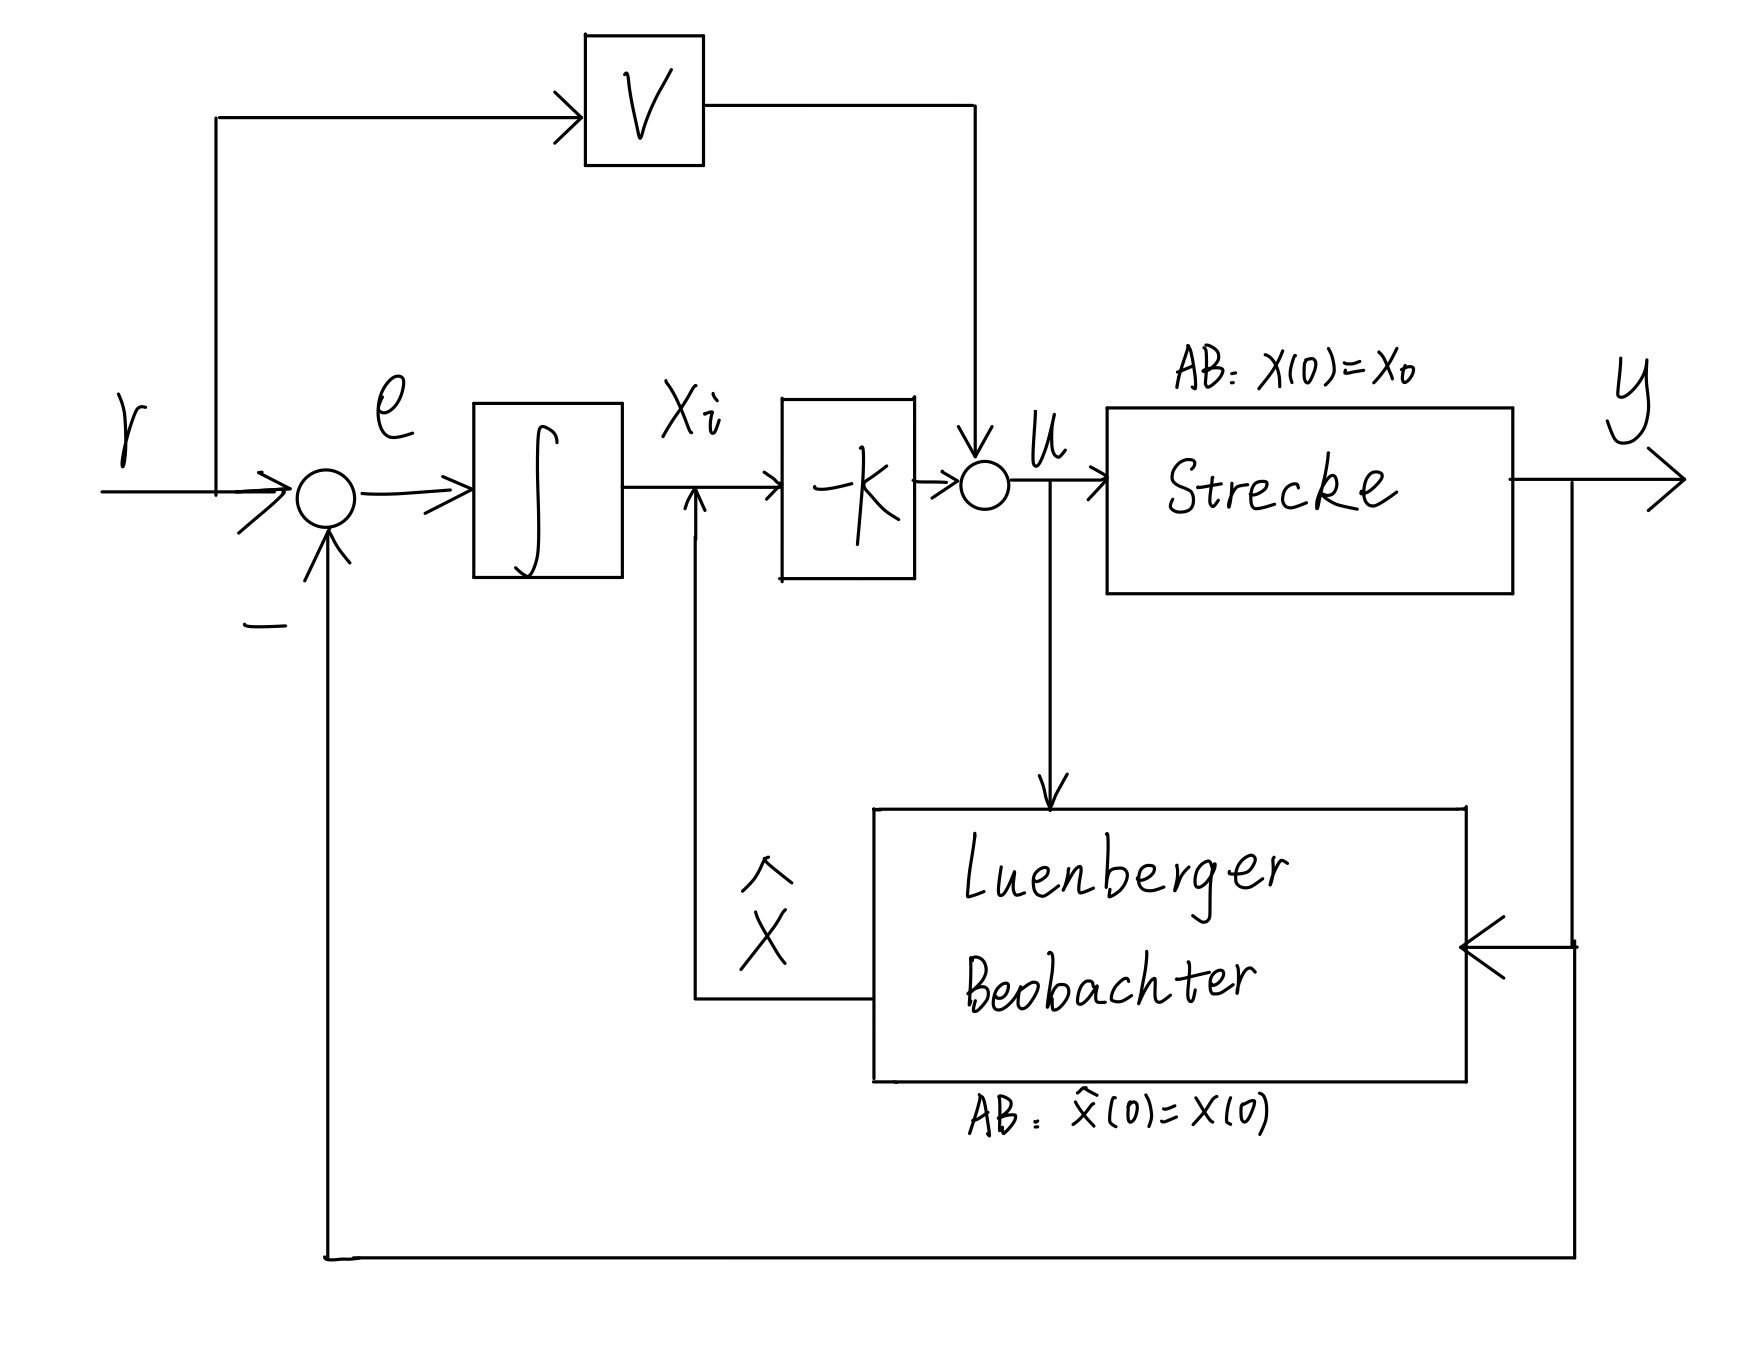
\includegraphics[scale=0.14]{Regelstruktur des linearisierten Systems} 
		\caption{Regelstruktur des linearisierten Systems}\label{fig:Regelstruktur des linearisierten Systems}
	\end{center}
\end{figure}\\
Die Reglerstruktur für das nichtlineare Modell und Black Box Modell stellt sich wie folgend dar(Abbildung \ref{fig:Reglerstruktur für das nichtlineare Modell und Black Box Modell}):\\
\begin{figure} [h]
	\begin{center} 
		\includegraphics[scale=0.18]{Reglerstruktur für das nichtlineare Modell und Black Box Modell} 
		\caption{Reglerstruktur für das nichtlineare Modell und Black Box Modell}\label{fig:Reglerstruktur für das nichtlineare Modell und Black Box Modell}
	\end{center}
\end{figure}\\

%%****************************************
Der LQI Regler wird mittels Matlab Befehl "lqi" angewendet. Für eine Strecke mit den Zustandsraumgleichungen:
 \begin{equation}{}
\begin{split}
	\left[\begin{array}{l}
		\Delta \dot{x} \\
		\Delta \dot{x}_{i}
	\end{array}
\right] =&\left[\begin{array}{c}
		A \Delta x+B \Delta u \\
		\Delta r-\Delta y
	\end{array}\right] \\
=&\underbrace{\left[\begin{array}{cc}
			A & 0 \\
			-C_{neu} & 0
		\end{array}\right]}_{A_{LQI}}\left[\begin{array}{c}
		\Delta x \\
		\Delta x_{i}
	\end{array}\right]+\underbrace{\left[\begin{array}{c}
			B \\
			0
		\end{array}\right]}_{B_{LQI}} \Delta u+\left[\begin{array}{c}
		0 \\
		I
	\end{array}\right] \Delta r
\end{split}
\end{equation}
$\Delta{x} \in  $\mathbb{R}^{6\times1}$ und $\Delta{x_{i}}$ ist der Integratorausgang für \\
Fehler $e$ \in $ \mathbb{R}^{2\times1}$. \\
\begin{equation}
	y_{neu}=\left[\begin{array}{c}
		\alpha\\\beta
	\end{array}\right]
\end{equation}
Die neue Matrix $A_{LQI}$ in jetztigen System lautet:
\begin{equation}
	A_{LQI}=\left[\begin{array}{llllllll}
		0 & 0 & 0 & 1 & 0 & 0 & 0 &0 \\
		0 & 0 & 0 & 0 & 1 & 0 & 0 &0 \\
			0 & 0 & 0 & 0 & 0 & 1 & 0 &0 \\
		0 & 0 & -0.6921 & 0 & 0 & 0 & 0 &0 \\
		0 & -0.0359 & 0 & 0 & 0 & 0 & 0 &0 \\
			0 & 0 & 0 & 0& 0 & 0 & 0 &0 \\
				-1 & 0 & 0 & 0 & 0 & 0 & 0 &0 \\
					0 & -1 & 0 & 0& 0 & 0 & 0 &0 
	\end{array}\right]
\end{equation}
Die Eingangsmatrix $B_{LQI}$:
\begin{equation}
	B_{LQI}=\left[\begin{array}{cc}
		\multicolumn{2}{c}{\multirow{4}{*}{\emph{O_{4,2}}}}\\
 			& \\
			& \\
	      0.5832& 0.5832\\
		5.5383& -5.5383\\
		\multicolumn{2}{c}{\multirow{2}{*}{\emph{O_{2,2}}}}\\
		
	\end{array}\right]
\end{equation}

Die neue Ausgangsmatrix C ergibt sich zu
\begin{equation}
	\begin{array}{l}
		C_{neu}=\left[\begin{array}{llllll}
			\multicolumn{2}{c}{I_2} \multicolumn{2}{c}{O_{2,3}}\\ 
%			1 & 0 & 0 & 0 & 0 & 0 \\
%			0 & 1 & 0 & 0 & 0 & 0 \\
		\end{array}\right] 
	\end{array}
\end{equation}

Die Matrix D lautet gleich wie früher:
\begin{equation}
		D= O_{3,2}	
\end{equation}


Denn wir brauchen nur die $\alpha$ und $\beta$ für Trajektorie, das bedeutet, 
\begin{equation}
	r=\left[\begin{array}{c}
		\alpha_{r}\\\beta_{r}
	\end{array}\right]
\end{equation}

Die Zustandsrückkopplungssteuerung hat die Form
\begin{equation}{}
	\Delta{u} = -K [\Delta{x}; \Delta {x_{i}}]
\end{equation}
%\begin{equation}
	%x=\left[\begin{array}{c}
	%	\alpha\\\beta\\\gamma\\\dot{\alpha}\\\dot{\beta}\\\dot{\gamma}\ 
	%\end{array}\right] 	
%\end{equation}

Und $K \in \mathbb{R}^{2\times8}$.\\

Das resultierende Gain $K _{LQI}(K _{LQR},K _{I})$ ist:\\[1.2 em]
%\begin{equation}{}
K_{LQR}=\left[\begin{array}{llllll}
		       -17.92& 8.33& 6.21 & -17.49 & 4.10& 1.27\\
			17.92& 8.33& -6.21 & 17.49 & 4.10& -1.27 
		\end{array}\Big] 
%K=[\begin{smallmatrix}
%	-2.4430& 1.6879& 2.2827& -3.8667 & 1.8413& 0.9551& 0.7071& -0.7071\\
%2.4430& 1.6879& -2.2827 & 3.8667&  1.8413&  -0.9551& -0.7071& -0.7071
\end{matrix}
%\end{equation}

%\begin{equation}
	\begin{array}{c}
		K _{I}=\left[\begin{array}{ll}
			6.3246& -3.1623\\
			-6.3246 &-3.1623
		\end{array}\right]
	\end{array}
%\end{equation}


Und der Vorfilter $V= -(C_{neu}(A-BK_{LQR})^{-1}B)^{-1} $ ist:

\begin{equation}
	\begin{array}{l}
		V=\left[\begin{array}{ll}
			-17.9241& 8.3613\\
			17.9241 &8.3613
		\end{array}\right]
	\end{array}
\end{equation}


Die Eigenwerte des geschlossenen Regelkreises ergeben sich zu:
\begin{equation}
	EW=\left[\begin{array}{c}
		-7.7685\\
		-0.4861+0.7260i\\
		-0.4861-0.7260i\\
		-0.9196+0.2243i\\
		-0.9196-0.2243i\\
		-0.6375+0.7327i\\
		-0.6375-0.7327i\\
	   -0.8754
	\end{array}\right]
\end{equation}
Die negativen Realteile der Eigenwerte zeigen alles asympotisch stabiles Verhalten des geschlossenen Regelkreises.

Der LQI-Regler wird durch Matlab-Befehl ''lqi'' angewandet. Dieses Steuergesetz stellt sicher, dass die Ausgabe y die Referenztrajektorie r gut verfolgt. Bei MIMO-Systemen entspricht die Anzahl der Integratoren der Dimension der Ausgabe y. [K, S, e] = lqi (SYS, Q, R, N) berechnet die optimale Verstärkungsmatrix K unter Berücksichtigung eines Zustandsraummodells SYS für die Matrizen Q, R, N (In unseren System wählen wir N=0). u und y sind absolute Werte für das linearisiertes Modell. Aber $\Delta u$ und $\Delta y$ sollen für das nichtlinearisiertes Modell angewendet werden.

%$Q=I_8$\\
%
%$R= I_2$\\

\begin{equation}

Q=\left[\begin{array}{llllllll}
	200& 0 & 0 & 0 & 0 & 0 & 0 & 0\\
	0 & 88 & 0 & 0 & 0 & 0 & 0 & 0\\
	0 & 0 & 20& 0& 0 & 0 & 0 & 0\\
    0 & 0 & 0 & 15 & 0 & 0 & 0 & 0\\
    0 & 0 & 0 & 0 & 5 & 0 & 0 & 0\\
    0 & 0 & 0 & 0 & 0 & 1 & 0 & 0\\
    0 & 0 & 0 & 0 & 0 & 0 & 80& 0\\
	0 & 0 & 0 & 0 & 0 & 0 & 0 & 20
\end{array}\right]
	\begin{array}{l}
		R=\left[\begin{array}{ll}
			1 & 0 \\
			0 & 1 
		\end{array}\right]
	\end{array}
\end{equation}

\subsection{Beobachterentwurf}
Da die Winkelgeschwindigkeiten des Helikopters nicht messbar sind, ist ein Beobachter erforderlich, welcher diese fehlenden Zustände schätzt. Der Luenberger Beobachter wird angewendet, um die Zustände zu rekonstruieren. Die Pole des Beobachters wurden nach diese Befehl: $p= min (real(EW))*3 $ ausgewählt. Die Pole p des Systems lautet:
\begin{equation}
	p =\left[\begin{array}{c}
		-23,-23.1,-23.2,-23.3,-23.4,-23.5
	\end{array}\right] ^{T}
\end{equation}

Und das resultierende Gain L vom Beobachter ist:
\begin{equation}
	L=\left[\begin{array}{lll}
		46.9000& 0 & 0 \\
		0 & 46.3000& 0 \\
		0 & 0 & 46.3000\\
		549.9000 & 0 & -0.6921 \\
		0 & 535.8841 & 0 \\
		0 & 0 & 535.9000\\
	\end{array}\right]
\end{equation}


%++++++Yuchan

%++++ JiaQi
\section{Referenztrajektorie}
Um die Aufgabe zu absolvieren, ist es notwendig, die Referenzsignale zu definieren. Diese Signale muss die vorgegebene Anforderungen erfüllen. Die Hauptaufgabe lassen sich wie Tabelle 1 definieren.
\begin{table}[H]
	\caption{Hauptaufgabe}
	\centering
	%\textcolor{red}{Tabelle mit Werten füllen + vervollständigen}
	%\label{table:parameters}	
	\begin{tabular}{|c|c|c|c|}
		\hline
		\bfseries Subtask & \bfseries Point & \bfseries $\alpha$ & \bfseries $\beta$ \\ \hline \hline
		Start	& $1$ & 0\degree & approx. -27\degree\\ \hline
		Cargo pick-up	& $2$ & 90\degree  &  approx. -22\degree  \\ \hline
		Cargo deposition & $3$ & 450\degree&  approx. -22\degree  \\ \hline
		Finish(landing) & $1$ & 0\degree &  approx. -27\degree  	\\ \hline
	\end{tabular}
\end{table}

Außerdem ist die Mindestflughöhe von Steigwinkel $\beta$ gleich $-7.5\degree$. Weil der Nickwinkel $\gamma$ nicht berücksichtigt wird, ist es nur notwendig, Referenzsignale für Schwenkwinkel $\alpha$ und Steigwinkel $\beta$ zu definieren. Die Trajektorie soll in einige Abschnitte unterteilt werden, in denen jeweils ein Zustand verändert wird. Es gibt verschiedene Möglichkeiten, wie z.B. Sprünge, Rampen, trigonometrische Funktionen(wie $\sin$ und $\cos$) oder Polynome n-ten Grades, um die Zustandsänderung bei jedem Abschnitt darzustellen. Hier wurden Sinus-Funktionen mit verschiedenen Zeitpunkten implementiert. Durch Phasenverschiebung ($\pi/2$) können die steigenden Sinus-Signale und die fallenden Sinus-Signale unterscheidet werden. Die steigenden Signale werden durch
\begin{equation}
    S_{steig}=Z \pm Zsin(\frac{2\pi(t-T_{start})}{2(T_{end}-T_{start})}-\pi/2)
\end{equation}
gegeben. Die fallende Signale werden durch
\begin{equation}
	S_{fall}=Z \pm Zsin(\frac{2\pi(t-T_{start})}{2(T_{end}-T_{start})}+\pi/2)
\end{equation}  
gegeben. Z ist die Amplitude bei jeder Abschnitt. $T_{start}$ ist der Startzeitpunkt von jedem Abschnitt. $T_{end}$ ist der Endzeitpunkt. Die Abschnitte lassen sich wie in Tabelle 2 definieren.
\begin{table}[H]
	\caption{Trajektorieabschnitte}
	\centering
	%\textcolor{red}{Tabelle mit Werten füllen + vervollständigen}
	%\label{table:parameters}	
	\begin{tabular}{|c|c|c|c|}
		\hline
		\bfseries Abschnitt & \bfseries $\alpha$ & \bfseries $\beta$ & \bfseries Aufgabe \\ \hline \hline
		1 & 0\degree & -27\degree & Start \\ \hline
		2 & 0\degree & -27\degree$\rightarrow$0\degree & /  \\ \hline
		3 & 0\degree & 0\degree & / \\ \hline
		4 & 0\degree$\rightarrow$90\degree & 0\degree  & / 	\\ \hline
		5 & 90\degree & 0\degree & /  	\\ \hline
		6 & 90\degree & 0\degree$\rightarrow$-22\degree & /  \\ \hline
		7 & 90\degree & -22\degree & Cargo Pick-up  	\\ \hline
		8 & 90\degree & -22\degree$\rightarrow$0\degree & /  \\ \hline
		9 & 90\degree & 0\degree & /  	\\ \hline
		10 & 90\degree$\rightarrow$450\degree & 0\degree & /  	\\ \hline
		11 & 450\degree & 0\degree & / 	\\ \hline
		12 & 450\degree & 0\degree$\rightarrow$-22\degree & /  	\\ \hline
		13 & 450\degree & -22\degree & Cargo deposition  	\\ \hline
		14 & 450\degree & -22\degree$\rightarrow$0\degree & /  	\\ \hline
		15 & 450\degree & 0\degree & /  	\\ \hline
		16 & 450\degree$\rightarrow$0\degree & 0\degree & /  	\\ \hline
		17 & 0\degree & 0\degree & /  	\\ \hline
		18 & 0\degree & 0\degree$\rightarrow$-27\degree & /  	\\ \hline
		19 & 0\degree & -27\degree & Finish(landing)  	\\ \hline
	\end{tabular}
\end{table}
 
Fig. 6 und 7 zeigen die Solltrajektorie in $\alpha$ und $\beta$ Richtung.


\begin{figure}[ht]
	\begin{center} 
		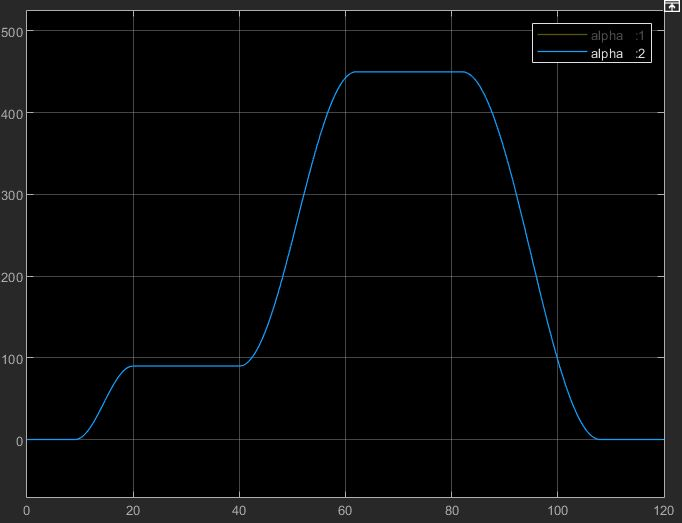
\includegraphics[scale=0.55]{alphasoll} 
		\caption{Sollsignal von $\alpha$}
		\label{fig:alphasoll}
	\end{center}
	
	\begin{center} 
		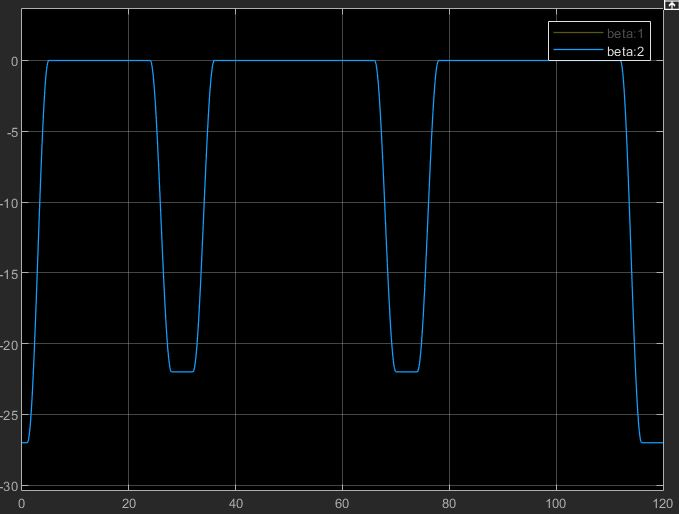
\includegraphics[scale=0.55]{betasoll} 
		\caption{Sollsignal von $\beta$}
		\label{fig:betasoll}
	\end{center}
\end{figure}

%\section{LQI-Regler}


\section{Simulationsergebnisse}

Nach dem Entwurf des Reglers wurde das System mit dem Black Box Modell getestet. Bei dem Black Box Modell musste die Vorzeichen von $\alpha$, $\beta$, und $\gamma$ beachtet. Wenn das Vorzeichen falsch sind, funktioniert der Regler schlecht. Die Solltrajektorie wurde an das System in Simulink angeschlossen, um die Funktion des Regler zu prüfen. Nach Auswahl passender Parameter könnte die Gesamtaufgabe unter 120s gelöst werden. In Fig.8 und 9 sind die Verläufe des Schwenkwinkelsignals($\alpha$) und des Steigwinkelsignals($\beta$). Der Signalverlauf der Solltrajektorie sind in den Abbildungen mit blau gekennzeichnet, während die geregelte Strecke in gelb gekennzeichnet ist. Aus den Abbildungen sieht man deutlich, dass das Verhalten des Reglers stark ist.

\begin{figure}[ht]
\begin{center} 
	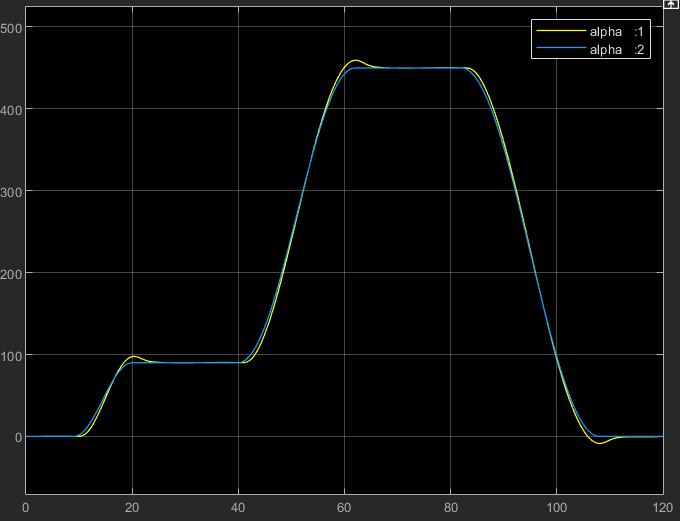
\includegraphics[scale=0.55]{alpha_final} 
	\caption{Ergebnis des Black Box Modells in $\alpha$}
	\label{fig:alpha_bbm}
\end{center}

\begin{center} 
	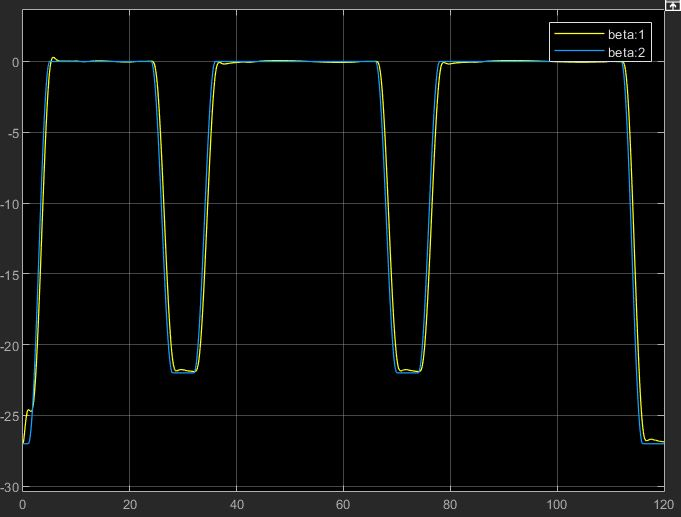
\includegraphics[scale=0.55]{beta_final} 
	\caption{Ergebnis des Black Box Modells in $\beta$}
	\label{fig:beta_bbm}
\end{center}

\end{figure}

\section{Fazit}
%In diesem Protokoll stellen wir unsere Arbeit für das Praktikum Konzept der Regelungstechnik vor, in der wir einen beobachterbasierten LQI-Regler für den 3-DOF Helikopter entworfen haben.  Wir verwendeten den systematischen Ansatz zur Lösung allgemeiner Regelungsprobleme. 

Entscheidende Schritte in der Reglerentwurf waren die Modellierung des Systems, die Wahl der Regelstruktur und des eigentlichen Reglertyps und schließlich die Implementierung und Validierung des entworfenen Reglers. Außerdem ist eine ordentliche Dokumentationen von Ergebnissen auch wichtig, da diese eine Richtlinie sind. Die Betreuung der Tutoren während des Praktikums war sehr hilfreich. Zusammengefasst, wir habe viele praktische Erfahrungen gesammeln können die wir auf weitere Aspekte im Studium sowie im Berufsleben anwenden können.
%\bibliographystyle{alpha}        % Include this if you use bibtex 
%\bibliography{autosam}           % and a bib file to produce the 
%\bibliography{autosam}
                                 % bibliography (preferred). The
                                 % correct style is generated by
                                 % Elsevier at the time of printing.

\begin{thebibliography}{1}
	
\bibitem{handbook}Handbook Control of a 3-DOF Helicopter
\\ IST, University of Stuttgart, Germany
\\ Corona Edition Winter term 2020/21
	
\bibitem{Regelkreisstrukturen}Regelkreisstrukturen
\\ IST, University of Stuttgart, Germany	

	
	
	
\end{thebibliography}

%\appendix
\end{document}
